\documentclass[12pt,a4paper]{article}
\usepackage[utf8]{inputenc}
\usepackage[english]{babel}
\usepackage{graphicx}
\usepackage{booktabs}
\usepackage{caption}
\usepackage{geometry}
\usepackage{hyperref}
\usepackage{float}
\usepackage{pdflscape}
\usepackage{enumitem}

\geometry{
    margin=2.5cm,
    top=2.5cm,
    bottom=2.5cm
}

\captionsetup{font=small, labelfont=bf}
\renewcommand{\thefigure}{S\arabic{figure}}
\renewcommand{\thetable}{S\arabic{table}}
\setlength{\parindent}{0pt}
\setlength{\parskip}{0.8ex}

\hypersetup{
    colorlinks=true,
    linkcolor=blue,
    urlcolor=blue
}

\begin{document}

% ============================================
% TÍTULO
% ============================================
\begin{center}
    {\LARGE \textbf{Supplementary Material}} \\[0.5cm]

\end{center}




\section{Supplementary Text}



\newpage

\section{Supplementary Tables}

\begin{table}[H]
\centering
\caption{\textbf{M9 minimal medium as imposed on every model.} Exchange reaction bounds in mmol~gDW$^{-1}$~h$^{-1}$, following Hao et al. (2013); negative lower bounds permit uptake. Applying one identical medium is what makes the models comparable, since each reconstruction otherwise ships with its own bounds. The ammonia cap of 5 matters most for interpretation: nitrogen, not carbon or oxygen, is what limits growth once glucose is supplied in excess, which is why the predicted growth curves saturate near 0.62~h$^{-1}$. It is also the bound on which the GEMs themselves disagree most, only three of the seven being distributed with this value while the rest ship ammonia at 100 mmol~gDW$^{-1}$~h$^{-1}$ or effectively unlimited, so imposing it uniformly is a modelling choice rather than a neutral default. In the glucose-uptake scan the oxygen bound is released so that respiration is not throttled independently of the carbon source.}
\begin{tabular}{l r r}
\toprule
\textbf{ID} & \textbf{LOWER\_BOUND} & \textbf{UPPER\_BOUND} \\
\midrule
EX\_h2o\_e   & -1000 & 1000 \\
EX\_o2\_e    & -18   & 0    \\
EX\_pi\_e    & -5    & 1000 \\
EX\_co2\_e   & -1000 & 1000 \\
EX\_nh4\_e   & -5    & 1000 \\
EX\_so4\_e   & -5    & 1000 \\
EX\_ca2\_e   & -1000 & 1000 \\
EX\_h\_e     & -1000 & 1000 \\
EX\_k\_e     & -1000 & 1000 \\
EX\_glc\_\_D\_e & -8.7 & 1000 \\
EX\_mg2\_e   & -1000 & 1000 \\
EX\_na1\_e   & -1000 & 1000 \\
EX\_fe3\_e   & -1000 & 1000 \\
EX\_fe2\_e   & -1000 & 1000 \\
\bottomrule
\end{tabular}
\label{tab:exchange_bounds}
\end{table}

\newpage

\begin{landscape}
\begin{table}[H]
\centering
\caption{\textbf{Network topology per model, from the MEMOTE reports} (Lieven et al., 2020). These counts describe structural integrity rather than predictive ability, and they are one component of the quality scores returned by MEMOTE. Blocked reactions, orphan and dead-end metabolites indicate portions of a network that can carry no flux and therefore contribute nothing to any simulation; stoichiometrically balanced cycles indicate thermodynamically infeasible loops. The pattern to note is that the newer and larger reconstructions do not have fewer such defects: iBsu1209 and the pangenome-derived Submodel carry the most blocked reactions and dead ends, while iYO844, the oldest and smallest model, carries among the fewest. Genes without gene--protein--reaction associations are genes the model contains but cannot use, which caps how much of the genome a gene essentiality analysis can cover, the lack of these GPR associations is prevented this analysis with the Submodel. ``ERRORED'' indicates the corresponding MEMOTE test did not return a value.}
\resizebox{\linewidth}{!}{%
\begin{tabular}{l*{10}{r}}
\toprule
\textbf{Metric} & \textbf{iYO844} & \textbf{iBsu1103} & \textbf{iBsu1103v2} & \textbf{iBsu1147} & \textbf{eciYO844} & \textbf{iBsu1209} & \textbf{iBB1018} & \textbf{iBsu1147R} & \textbf{ecBSU1} & \textbf{Submodel} \\
\midrule
Universally Blocked Reactions & 291 & 419 & 391 & 377 & 293 & 841 & 282 & 805 & ERRORED & 826 \\
Orphan Metabolites & 49 & 58 & 58 & 67 & 48 & 84 & 79 & 67 & 67 & 185 \\
Dead-end Metabolites & 122 & 96 & 94 & 104 & 124 & 145 & 93 & 105 & 108 & 255 \\
Stoichiometrically Balanced Cycles & 21 & 331 & 307 & 76 & 17 & 178 & 34 & 80 & ERRORED & 129 \\
Metabolite Production in Complete Medium & 107 & 310 & 294 & 358 & 108 & 506 & 301 & 371 & ERRORED & 681 \\
Metabolite Consumption in Complete Medium & 262 & 380 & 352 & 446 & 264 & 860 & 21 & 740 & ERRORED & 846 \\
Genes without GPR Associations & 117 & 244 & 249 & 193 & 117 & 172 & 1 & 193 & 323 & 1756 \\
\bottomrule
\end{tabular}%
}
\label{tab:network_topology}
\end{table}
\end{landscape}

\newpage
\newpage

\begin{table}[H]
\centering
\caption{\textbf{Terminal oxidase usage before and after deletion of the caa$_3$ oxidase}, under M9 minimal medium with glucose. Fluxes in mmol~gDW$^{-1}$~h$^{-1}$, growth rate in h$^{-1}$; the \textit{other} column collects any remaining oxygen-consuming reaction. Cytochrome \textit{bd} carries no flux in any model and is omitted. Six of the seven models respire through the caa$_3$ branch, which is the most energetically favourable of the four terminal oxidases of \textit{B. subtilis} but is repressed by catabolite control protein A during growth on glucose. Deleting it does not merely remove capacity: every affected model transfers its respiratory flux to the aa$_3$-600 quinol oxidase, the route that carries the main electron flow in glucose-grown cells, and the predicted growth rate falls accordingly. iBsu1147 already uses that route before any deletion and is unaffected. The Submodel, which contains additional oxidases absent from the others, switches to one of those instead.}
\label{tab:oxidase_flux}
\begin{tabular}{lrrrrrrrr}
\toprule
& \multicolumn{4}{c}{\textbf{Wild type}} & \multicolumn{4}{c}{\textbf{caa$_3$ knockout}} \\
\cmidrule(lr){2-5}\cmidrule(lr){6-9}
\textbf{Model} & \textbf{caa$_3$} & \textbf{aa$_3$-600} & \textbf{other} & \textbf{$\mu$}
               & \textbf{caa$_3$} & \textbf{aa$_3$-600} & \textbf{other} & \textbf{$\mu$} \\
\midrule
iYO844 & 35.9 & 0.0 & 0.1 & 0.61 & 0.0 & 35.9 & 0.1 & 0.42 \\
iBsu1147 & 0.0 & 35.9 & 0.1 & 0.59 & 0.0 & 35.9 & 0.1 & 0.59 \\
eciYO844 & 35.9 & 0.0 & 0.1 & 0.60 & 0.0 & 35.9 & 0.1 & 0.41 \\
iBB1018 & 25.7 & 10.3 & 0.0 & 0.63 & 0.0 & 36.0 & 0.0 & 0.47 \\
iBsu1147R & 35.9 & 0.0 & 0.1 & 0.55 & 0.0 & 35.9 & 0.1 & 0.42 \\
ecBSU1 & 32.4 & 0.0 & 1.8 & 0.55 & 0.0 & 35.9 & 0.1 & 0.42 \\
Submodel & 34.8 & 0.0 & 0.0 & 0.62 & 0.0 & 0.0 & 36.0 & 0.48 \\
\bottomrule
\end{tabular}
\end{table}


\section{Supplementary Figures}

\begin{figure}[H]
\centering
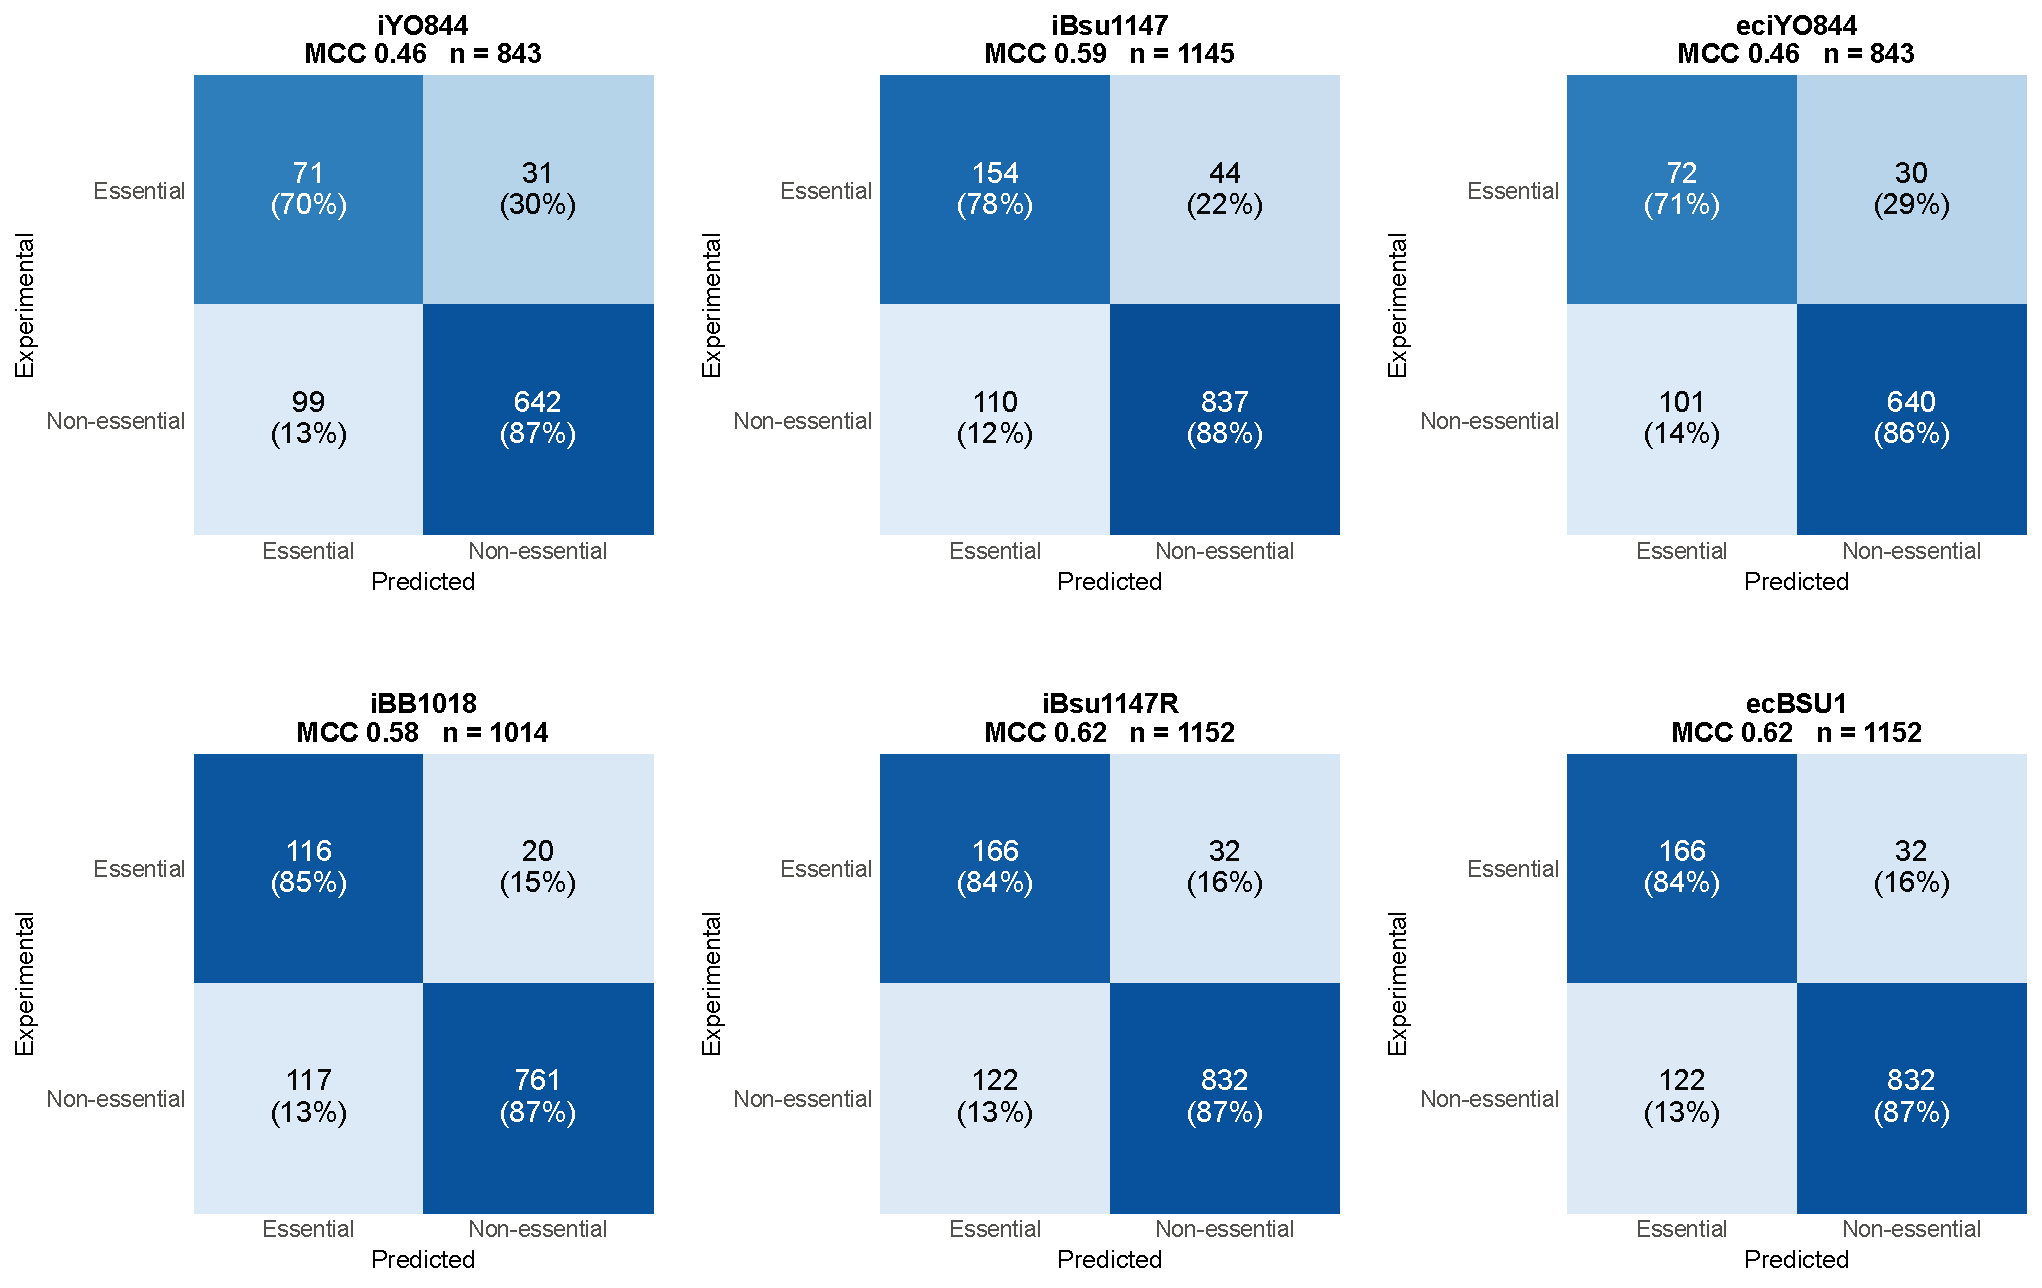
\includegraphics[width=\textwidth]{../analysis/results/figures/Fig_confusion_matrices.pdf}
\caption{\textbf{Gene essentiality predictions against experimental data, per model.} Rows give the experimental call and columns the prediction. Each panel is headed by the Matthews correlation coefficient and the number of genes matched. All six models err in the same direction. The upper-left cell is consistently large --- most genes that are truly essential are found --- but so is the lower-left, meaning many dispensable genes are also called essential. This over-prediction is the expected behaviour of a purely stoichiometric model, in which deleting any gene that blocks a biomass precursor is lethal, with no isoenzyme regulation or metabolic rerouting available to rescue it.}
\label{fig:confusion_matrices}
\end{figure}

\newpage

\begin{figure}[H]
\centering
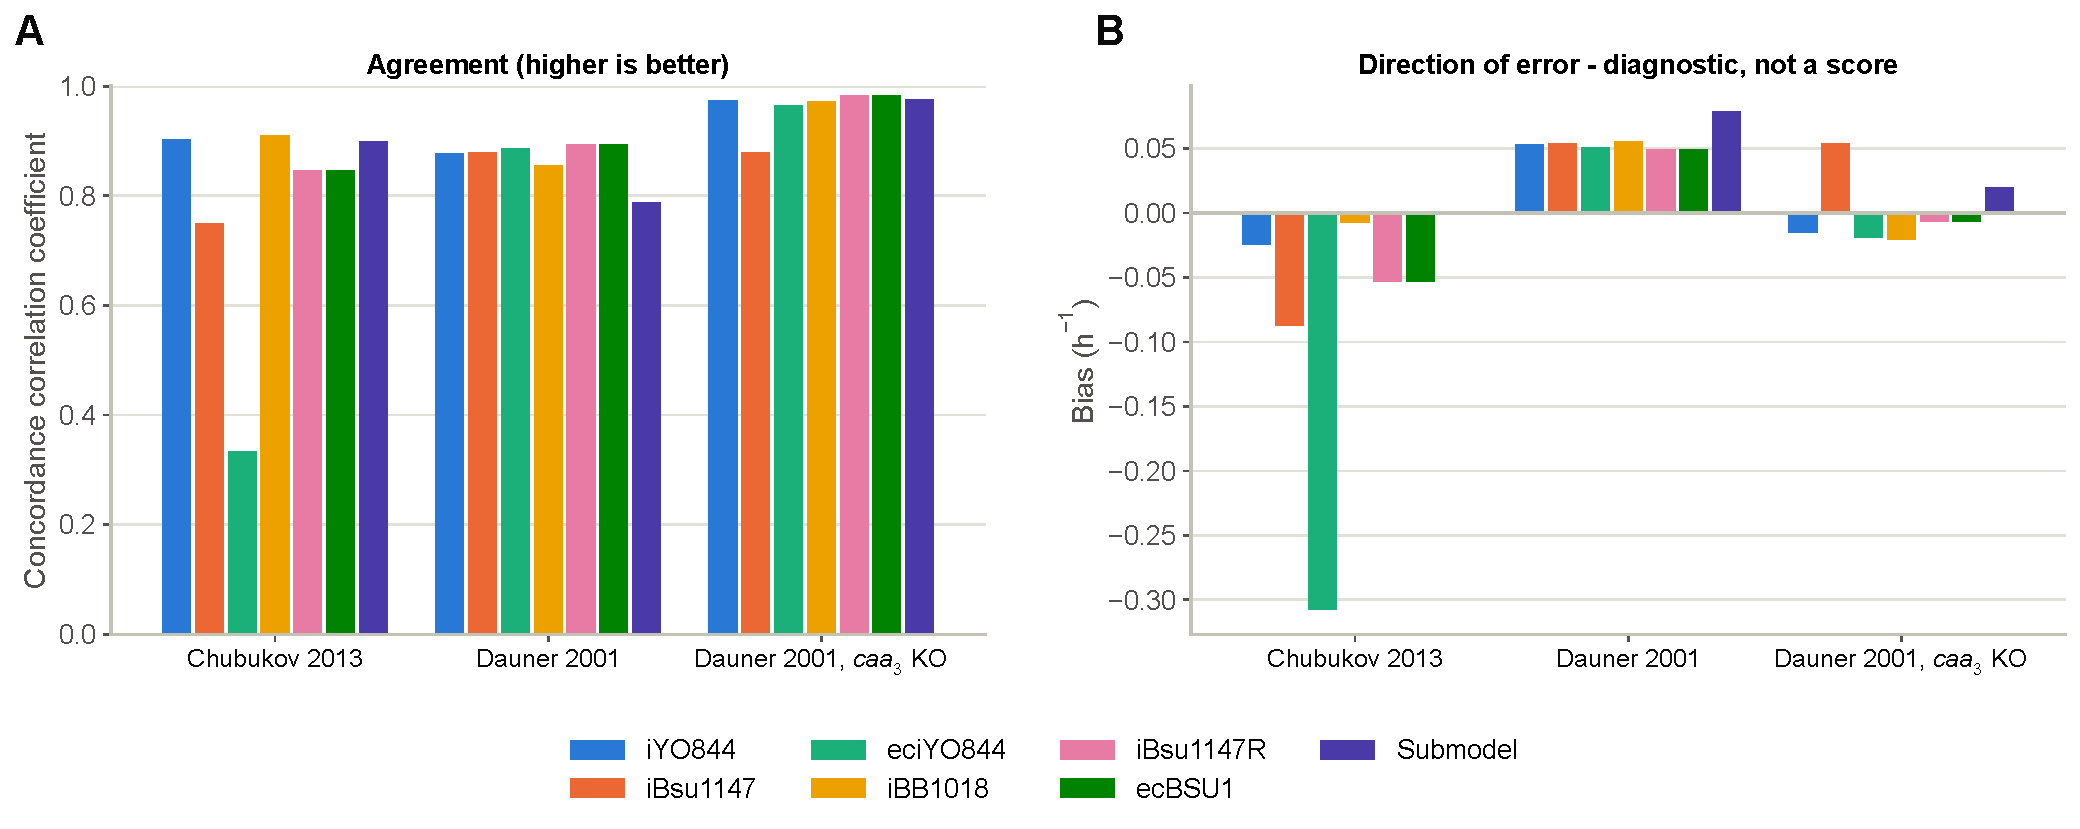
\includegraphics[width=\textwidth]{../analysis/results/figures/Plot_growth_fit_metrics.pdf}
\caption{\textbf{Fit statistics for predicted growth rates, per model and experiment}. \textbf{(A)} Lin's concordance correlation coefficient, which measures agreement with the identity line and therefore penalizes a systematic offset and a difference in scale, unlike Pearson's correlation. Models agree closely with each other on the chemostat series, which therefore discriminates poorly between them, and diverge on the carbon-source experiment, where eciYO844 collapses because it fails to grow on six of the eight substrates. Deleting the cytochrome \textit{caa}$_3$ oxidase raises agreement for every model except iBsu1147, whose predictions are unchanged by the deletion. \textbf{(B)} Bias, the mean signed deviation in h$^{-1}$. The direction of error is a property of the condition rather than of the model: every model underestimates growth on the carbon sources and every model overestimates it on the chemostat series, and the knockout returns the latter slightly past zero rather than exactly to it. }
\label{fig:growth_fit_metrics}
\end{figure}

\newpage

\begin{figure}[H]
\centering
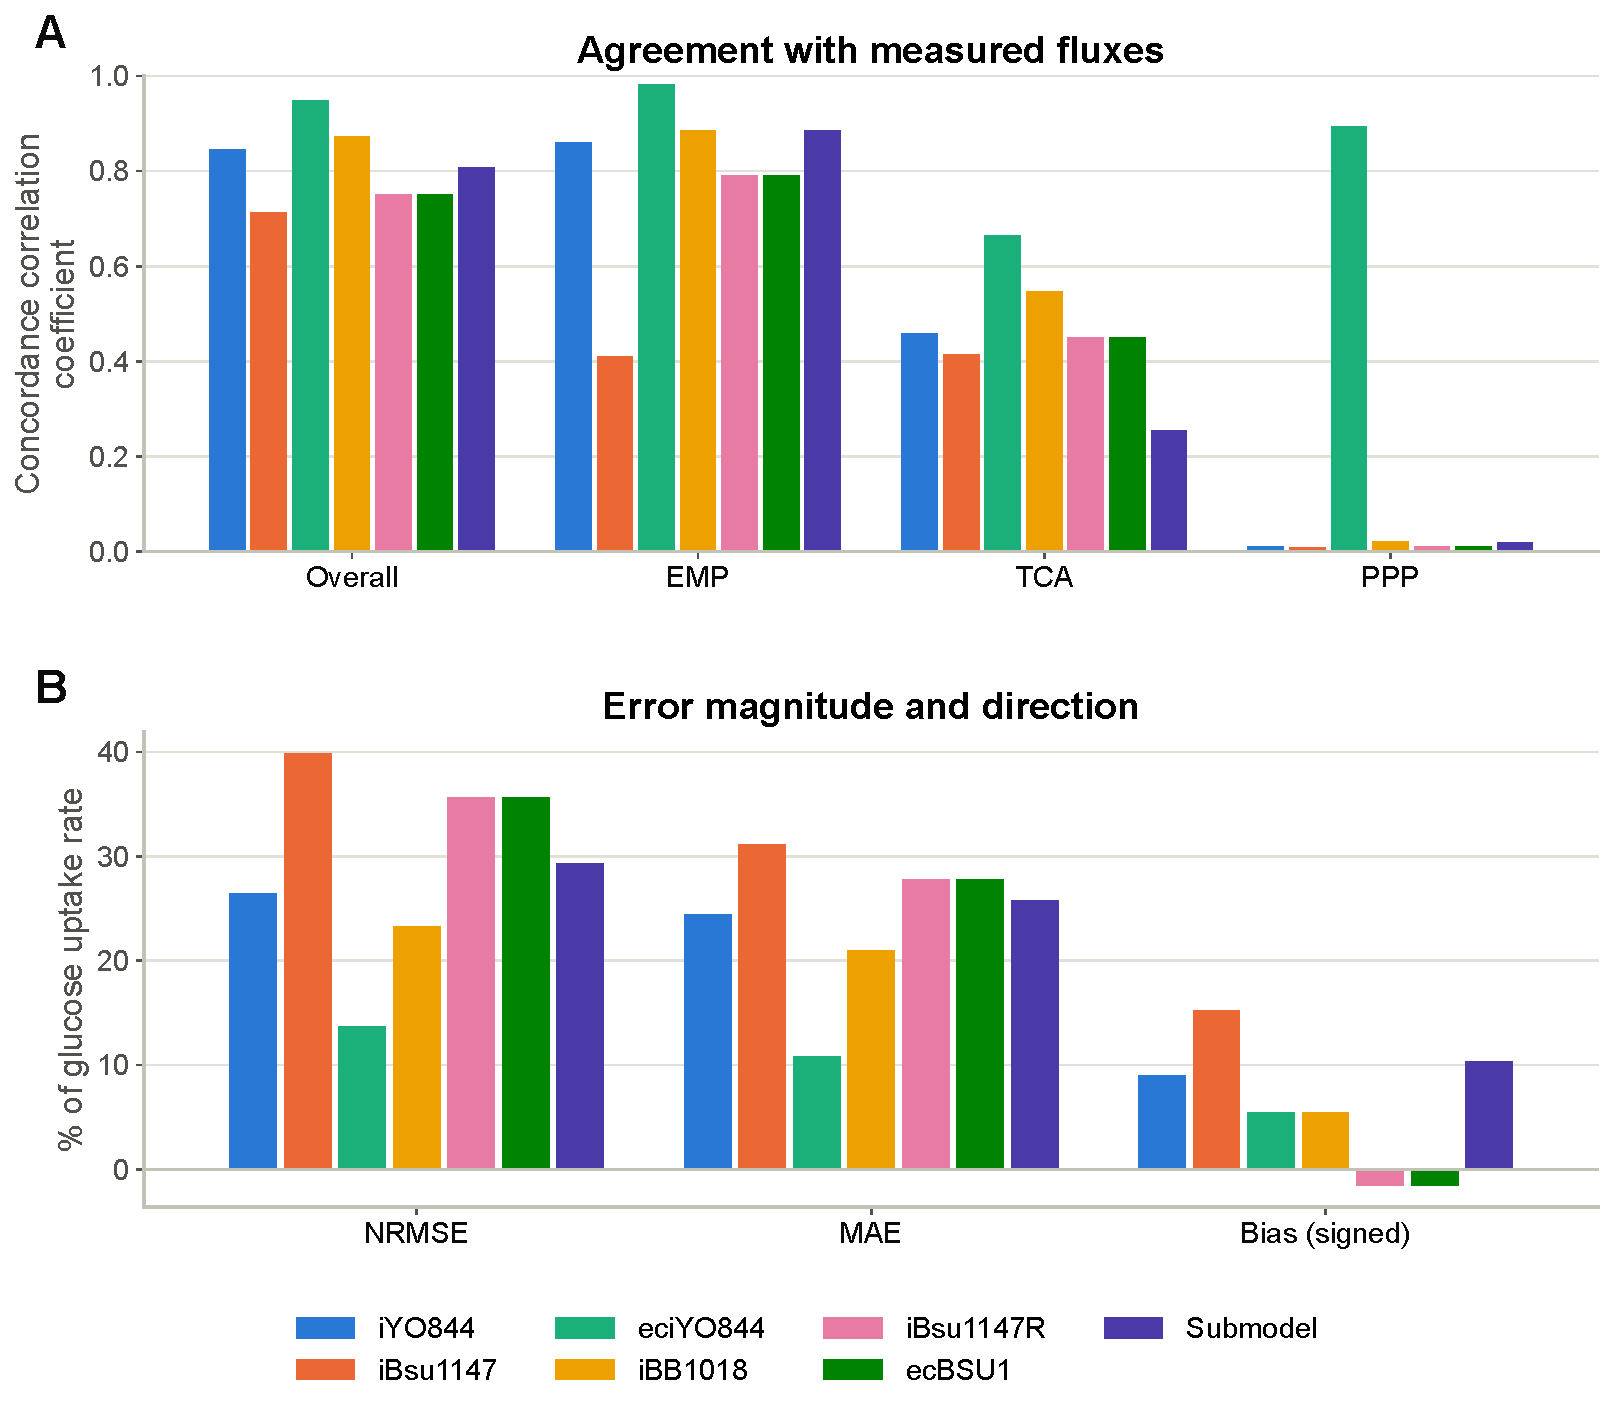
\includegraphics[width=\textwidth]{../analysis/results/figures/carbon_metabolism_flux_metrics.pdf}
\caption{\textbf{Agreement between predicted and measured central carbon fluxes, per model.} \textbf{(A)} Concordance correlation coefficient over the twenty stoichiometrically independent reactions, pooled and separately for each pathway.Glycolysis, which carries the largest fluxes and which every model reproduces well, conceals the fact that the oxidative pentose phosphate pathway is essentially inactive in six of the seven models. Only eciYO844 reproduces that branch, which is what places it first overall.  \textbf{(B)} Normalized root mean square error, mean absolute error and bias, all as a percentage of each model's realized glucose uptake rate.}
\label{fig:carbon_metabolism_flux_metrics}
\end{figure}

\newpage
\begin{figure}[H]
\centering
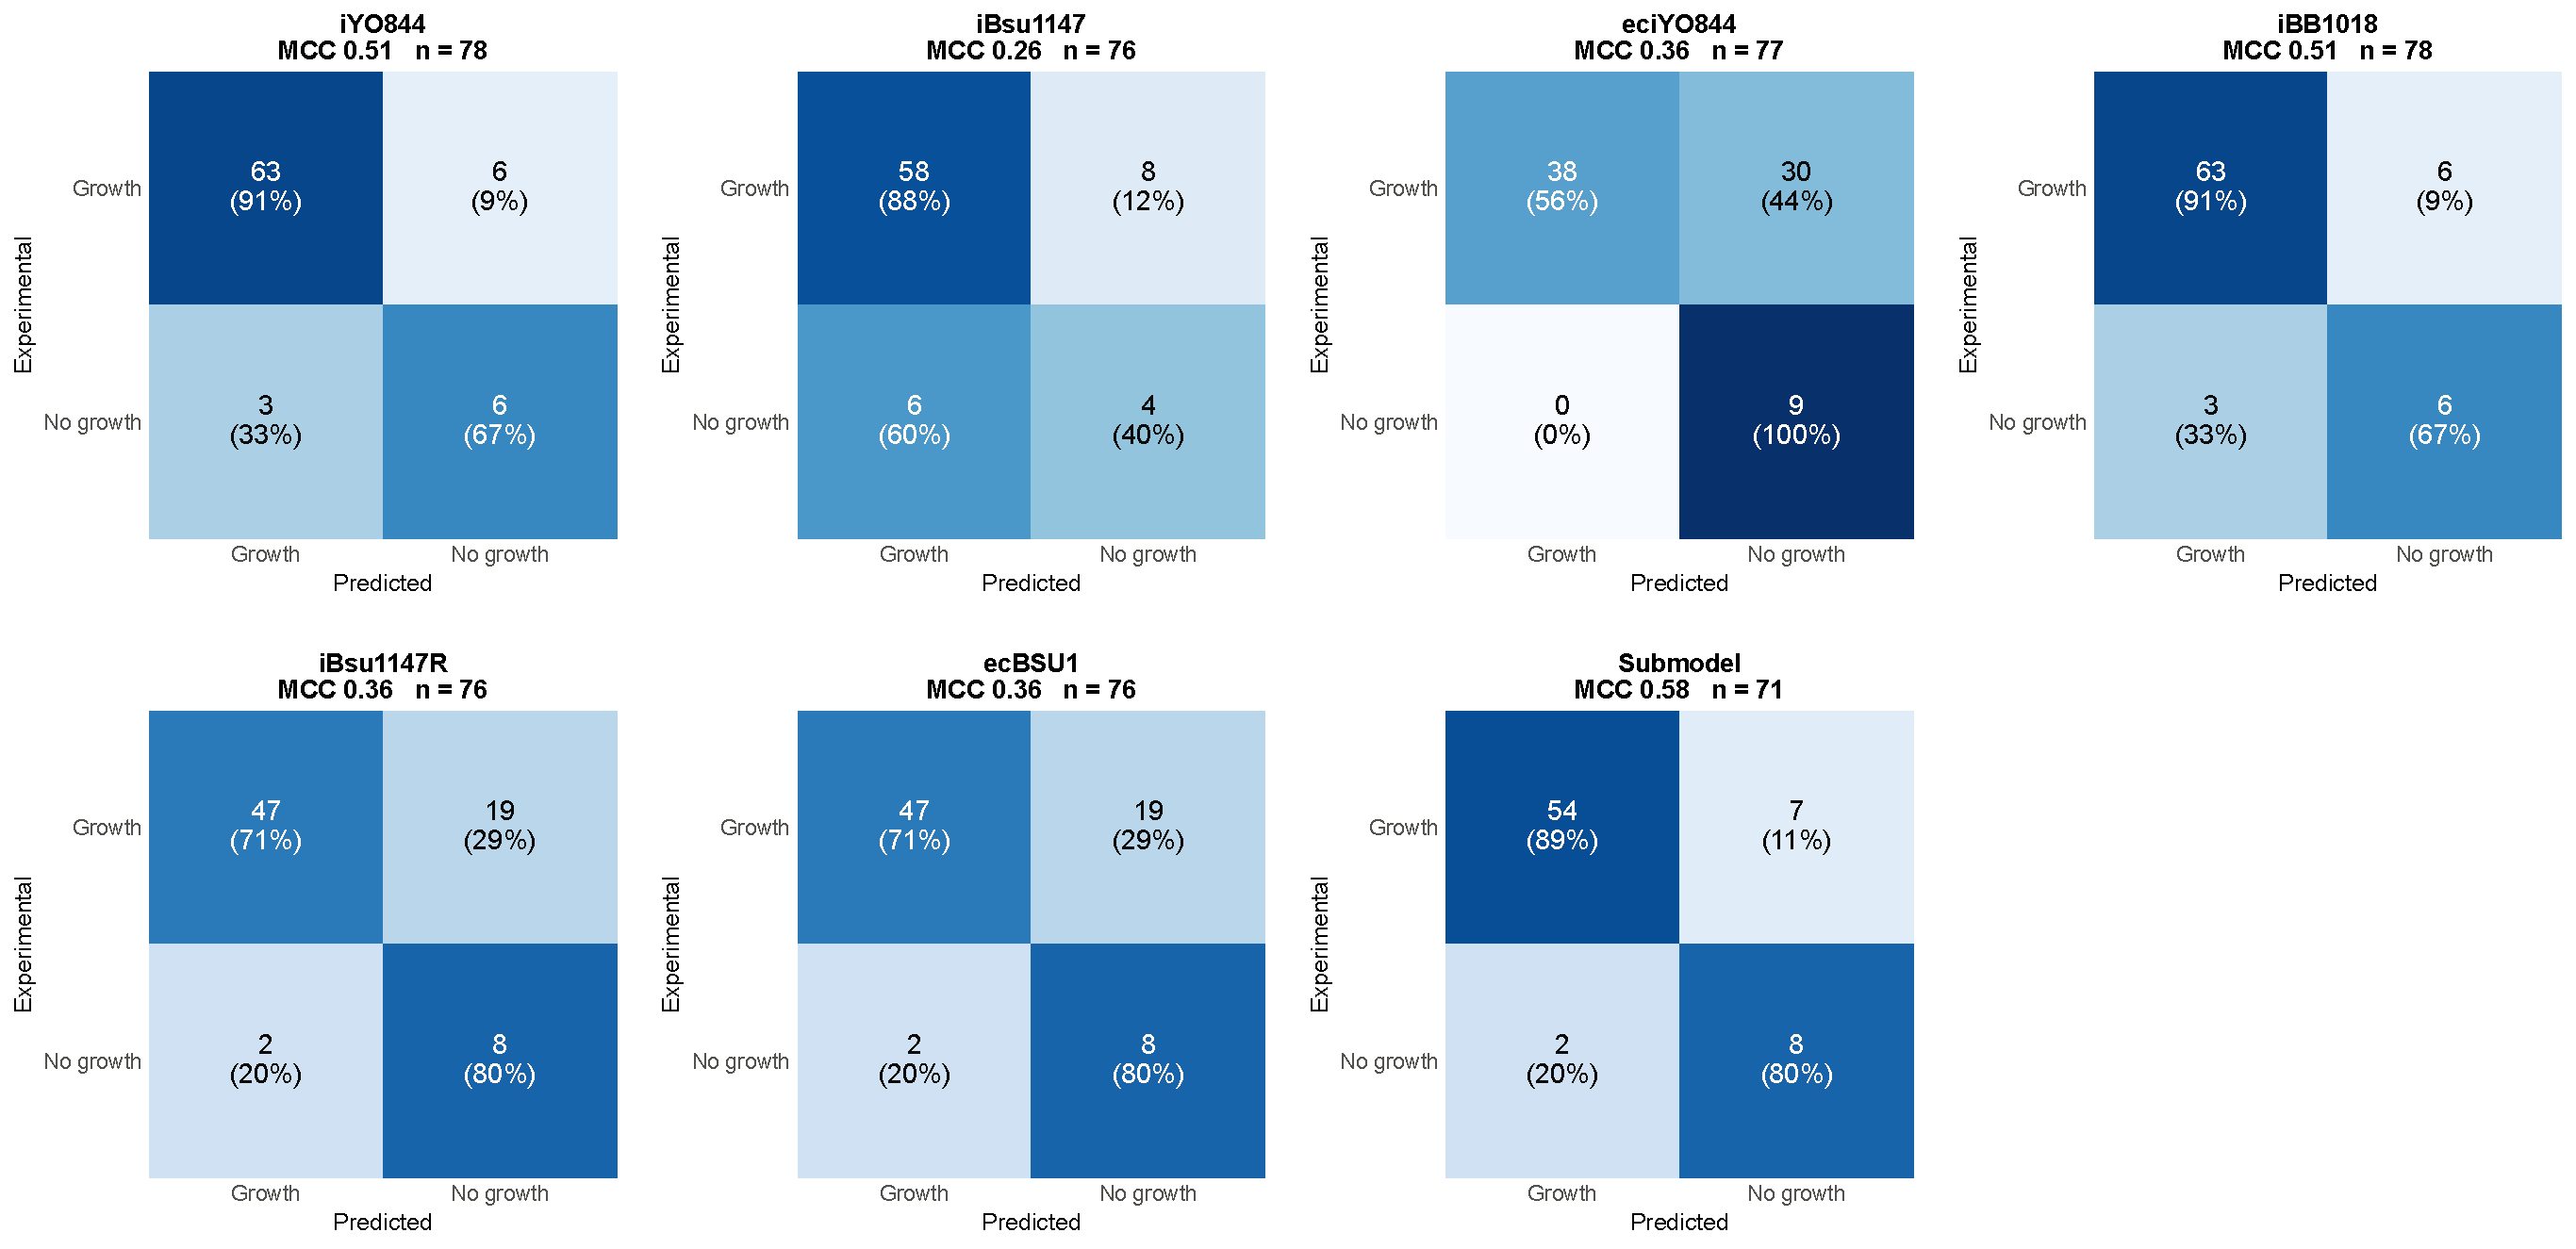
\includegraphics[width=\textwidth]{../analysis/results/figures/Fig_carbon_utilization_matrices.pdf}
\caption{\textbf{Carbon-source utilization predictions against Biolog phenotyping data} (Oh et al., 2007), per model. Each panel is headed by the Matthews correlation coefficient and the number of substrates that could be tested. iYO844, iBB1018 and the Submodel are permissive because they recover almost every substrate that supports growth, but a third of the substrates the organism cannot use are predicted to support growth anyway. eciYO844 behaves in exactly the reverse manner, with no false positives at all, missing 30 of the 68 substrates that do support growth. This is the same over-constrained behaviour that makes it the best predictor of intracellular fluxes.}
\label{fig:carbon_utilization_metrics}
\end{figure}

\newpage

\begin{figure}[H]
\centering
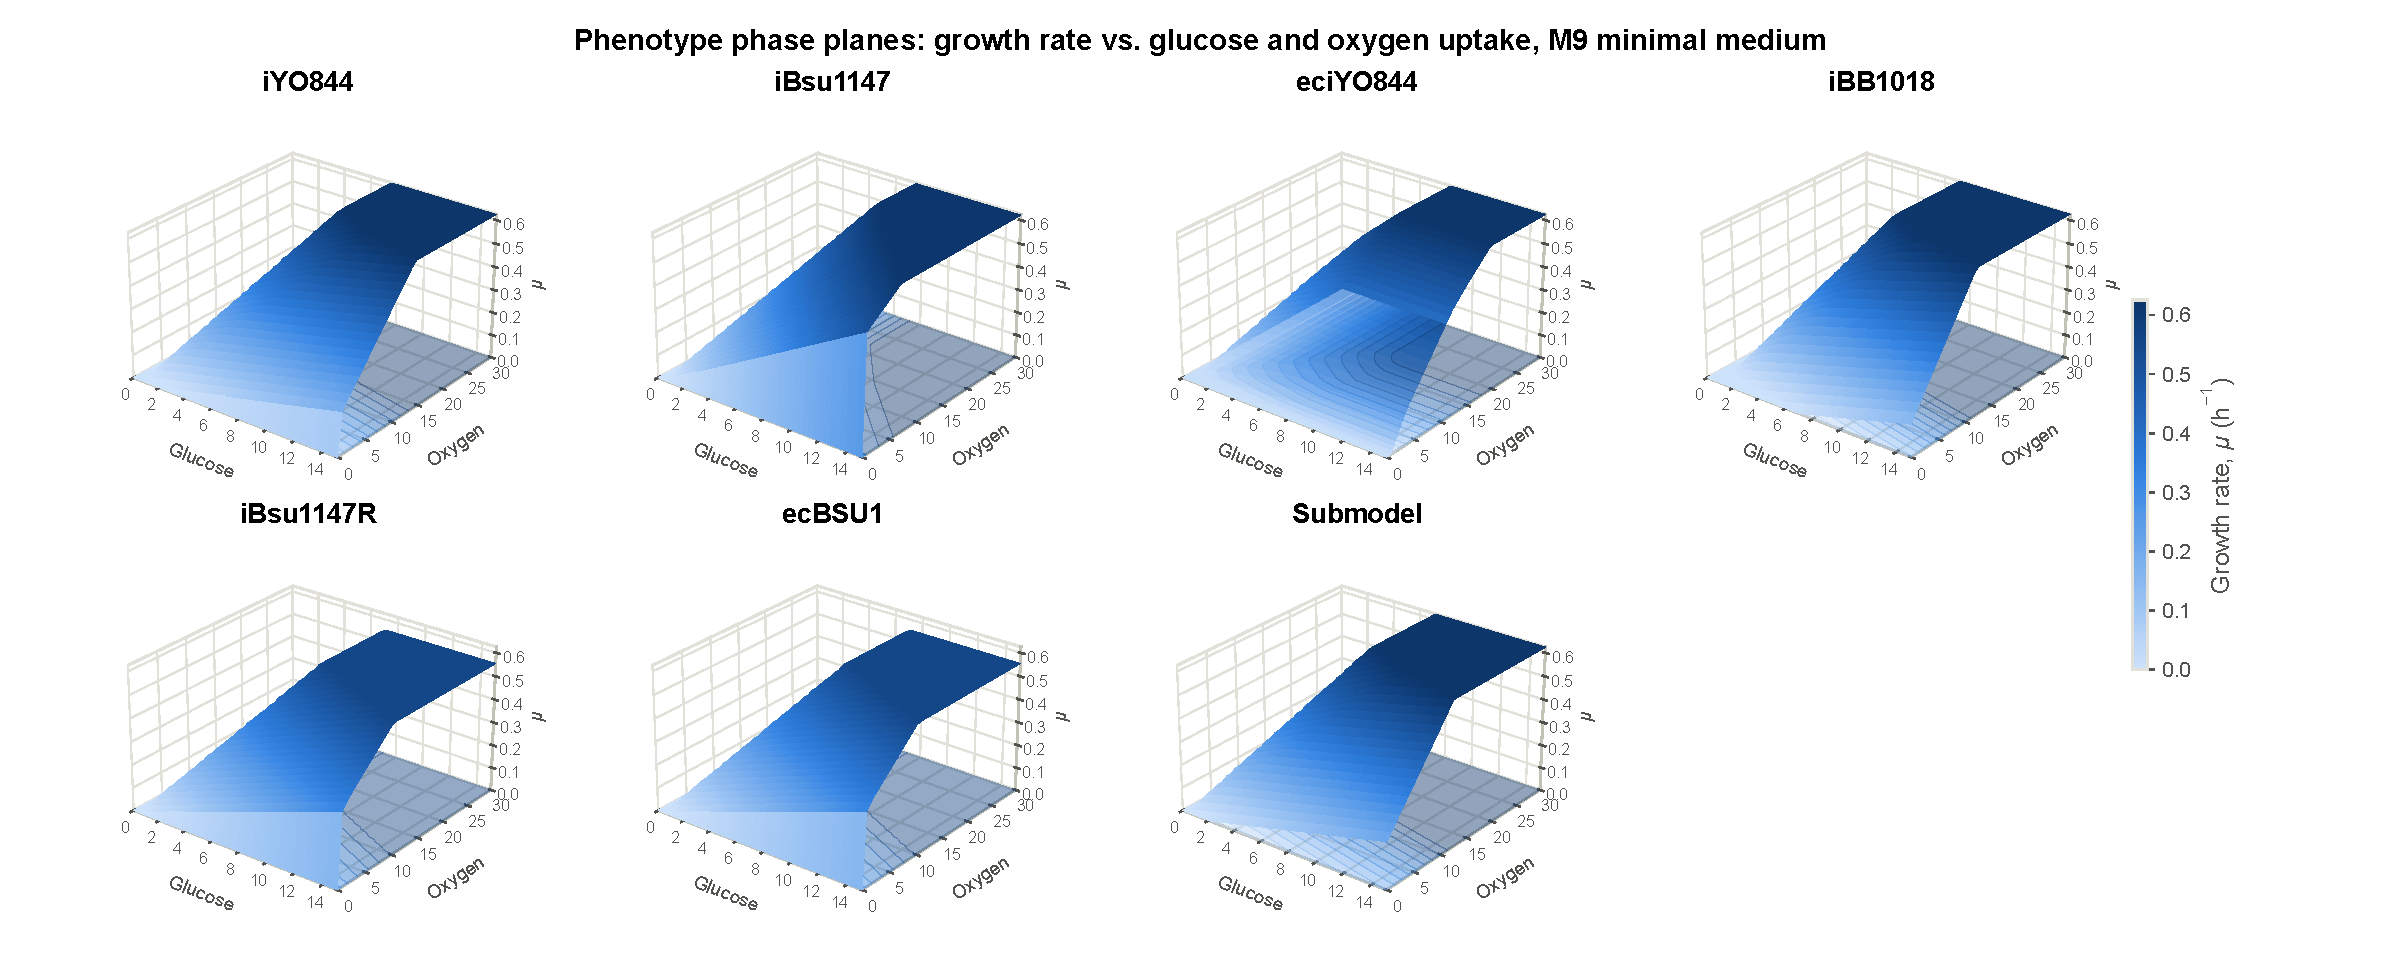
\includegraphics[width=0.95\textwidth]{../analysis/results/figures/3d_PhPP/PhPP_3D_all_models.pdf}
\caption{\textbf{Phenotype phase planes for glucose and oxygen uptake, per model.} Growth rate was recorded from FBA over a grid of glucose and oxygen uptake bounds, with all other exchange bounds held at their M9 values, following the two-substrate approach of Edwards, Ibarra and Palsson (2001). All panels share a common growth-rate scale. The surfaces rise along both axes and then flatten into a plane, and the position of that ceiling is informative. Growth becomes insensitive to further glucose and oxygen well inside the range scanned, because ammonia, capped at 5 mmol~gDW$^{-1}$~h$^{-1}$ becomes limiting instead. iBsu1147R and ecBSU1 produce indistinguishable surfaces, consistent with their identical behaviour in every other test.}
\label{fig:phpp_3d_all_models}
\end{figure}

\newpage

\section{References}

\begin{enumerate}[leftmargin=*]
\item Hao, T., Han, B., Ma, H., Fu, J., Wang, H., Wang, Z., Tang, B., Chen, T., \& Zhao, X. (2013). In silico metabolic engineering of \textit{Bacillus subtilis} for improved production of riboflavin, Egl-237, (R,R)-2,3-butanediol and isobutanol. \textit{Molecular BioSystems}, 9(8), 2034. \url{https://doi.org/10.1039/c3mb25568a}
\item Lieven, C., Beber, M. E., Olivier, B. G., et al. (2020). MEMOTE for standardized genome-scale metabolic model testing. \textit{Nature Biotechnology}, 38(3), 272--276. \url{https://doi.org/10.1038/s41587-020-0446-y}
\item Oh, Y.-K., Palsson, B. O., Park, S. M., Schilling, C. H., \& Mahadevan, R. (2007). Genome-scale reconstruction of metabolic network in \textit{Bacillus subtilis} based on high-throughput phenotyping and gene essentiality data. \textit{Journal of Biological Chemistry}, 282(39), 28791--28799. \url{https://doi.org/10.1074/jbc.m703759200}
\item Chubukov, V., Uhr, M., Le Chat, L., et al. (2013). Transcriptional regulation is insufficient to explain substrate-induced flux changes in \textit{Bacillus subtilis}. \textit{Molecular Systems Biology}, 9, 709. \url{https://doi.org/10.1038/msb.2013.66}
\end{enumerate}

\end{document}